\section{Scenarios}

\subsection{Introduction to MATSim Scenarios}

\begin{frame}
\frametitle{Scenarios}
\framesubtitle{Description of a Scenario}
\begin{columns}[T]

\column{7cm}

\begin{itemize}
  \item Parts of Scenario:
  \begin{itemize}
    \item Network: Road network
	\item Population: Description of agents
  \end{itemize}
  \item Configuration of scenario by XML--File
\end{itemize}

\column{5cm}
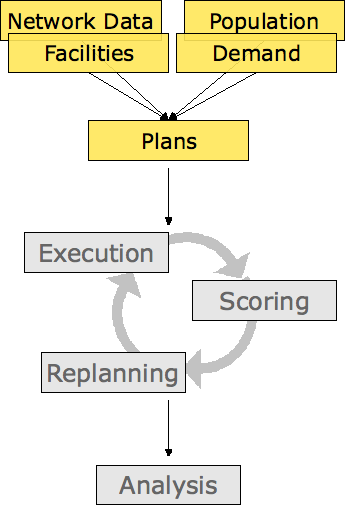
\includegraphics[width=4cm]{../graphics/overviewMatsimDemand.png}

\end{columns}

\end{frame}

\subsection{The Equil Scenario}


\begin{frame}[fragile]
\frametitle{Scenarios}
\framesubtitle{Equil Network}
\begin{itemize}
  \item Equil scenario:
  \begin{itemize}
  	\item \verb|./examples/equil/|
  \end{itemize}
  \item Start visualizer
  \begin{itemize}
  	\item Main method in \verb|org.matsim.utils.vis.netvis.NetVis|
  \end{itemize}
  \item Take a look at network
  \begin{itemize}
  	\item \verb|./examples/equil/network.xml|
  \end{itemize}
\end{itemize}
\end{frame}